%&pdflatex
\documentclass{standalone}
\usepackage{tikz}
\usetikzlibrary{arrows}
\usetikzlibrary{shapes}

\tikzstyle{startstop} = [rectangle, rounded corners, minimum width=2cm, minimum height=1cm,text centered, draw=black, fill=red!30, text width=2cm]
\tikzstyle{process} = [rectangle, minimum width=1cm, minimum height=1cm, text centered, draw=black, fill=orange!30, text width=2.5cm]
\tikzstyle{arrow} = [ultra thick,->,>=stealth]
\begin{document}

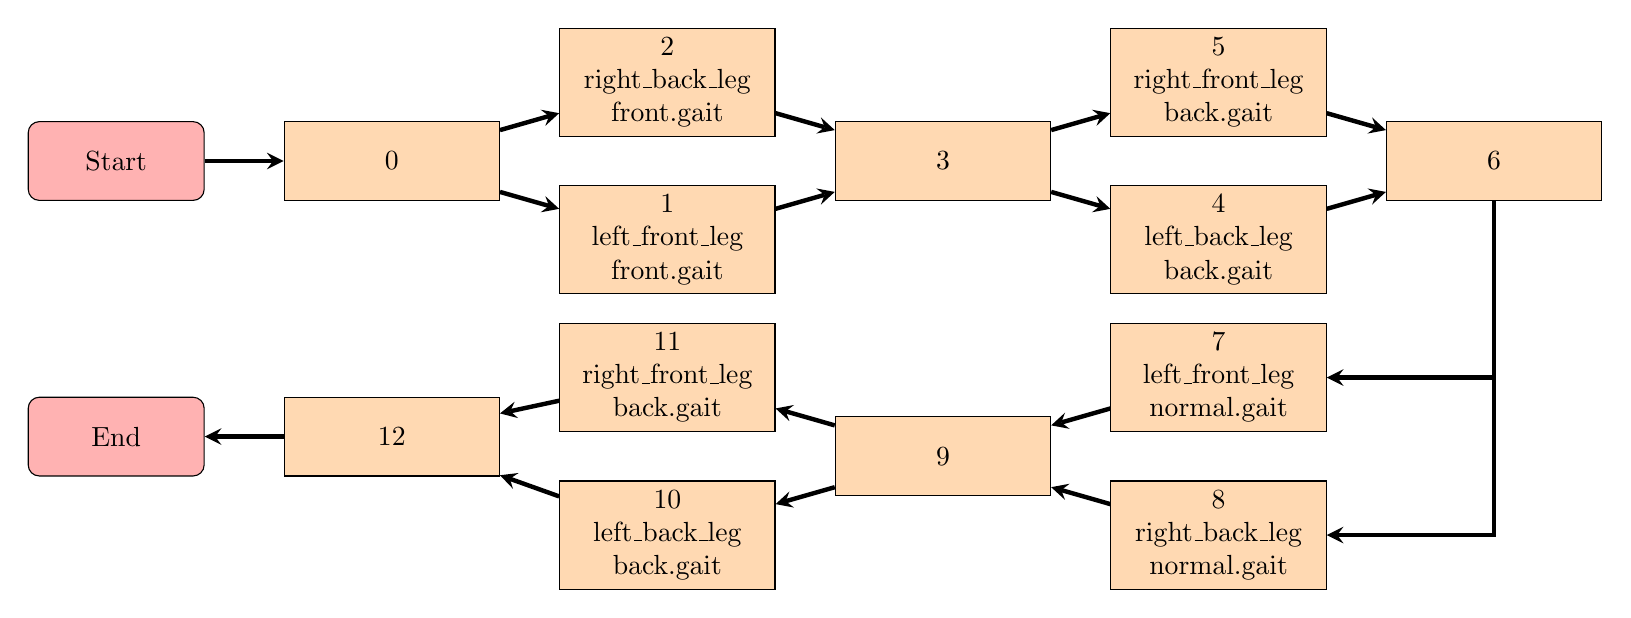
\begin{tikzpicture}[node distance=3.5cm]


\node [startstop] (start) {Start};
\node [process, right of = start] (s0) {0};
\node [process, right of = s0, yshift=-1cm] (s1) {1 \\ left\_front\_leg \\ front.gait};
\node [process, right of = s0, yshift=1cm] (s2) {2 \\ right\_back\_leg \\ front.gait};

\node [process, right of = s0, xshift=3.5cm] (s3) {3};
\node [process, right of = s3, yshift=-1cm] (s4) {4 \\ left\_back\_leg \\ back.gait};
\node [process, right of = s3, yshift=1cm] (s5) {5 \\ right\_front\_leg \\ back.gait};

\node [process, right of = s3, xshift=3.5cm] (s6) {6};
\node [process, below of = s4, yshift=1.75cm] (s7) {7 \\ left\_front\_leg \\ normal.gait};
\node [process, below of = s7, yshift=1.5cm] (s8) {8 \\ right\_back\_leg \\ normal.gait};

\node [process, below of = s3, yshift=-0.25cm] (s9) {9};
\node [process, left of = s9, yshift=-1cm] (s10) {10 \\ left\_back\_leg \\ back.gait};
\node [process, left of = s9, yshift=1cm] (s11) {11 \\ right\_front\_leg \\ back.gait};

\node [process, below of = s0, yshift=0cm] (s12) {12};

\node [startstop, below of = start, yshift=0cm] (end) {End};

\draw [arrow] (start) -- (s0);
\draw [arrow] (s0) -- (s1);
\draw [arrow] (s0) -- (s2);
\draw [arrow] (s1) -- (s3);
\draw [arrow] (s2) -- (s3);

\draw [arrow] (s3) -- (s4);
\draw [arrow] (s3) -- (s5);
\draw [arrow] (s4) -- (s6);
\draw [arrow] (s5) -- (s6);

\draw [arrow] (s6) |- (s7.east);
\draw [arrow] (s6) |- (s8.east);
\draw [arrow] (s7) -- (s9);
\draw [arrow] (s8) -- (s9);

\draw [arrow] (s9) -- (s10);
\draw [arrow] (s9) -- (s11);
\draw [arrow] (s10) -- (s12);
\draw [arrow] (s11) -- (s12);
\draw [arrow] (s12) -- (end);

\end{tikzpicture}

\end{document}



